\documentclass[a4paper, fontsize=11pt]{scrartcl} % A4 paper and 11pt font 
\usepackage[a4paper,left=3cm,right=2cm,top=2.5cm,bottom=2.5cm]{geometry}

\usepackage[T1]{fontenc} % Use 8-bit encoding that has 256 glyphs
\usepackage{fourier} % Use the Adobe Utopia font for the document - comment this line to return to the LaTeX default
\usepackage[spanish]{babel} % Spanish language/hyphenation
\selectlanguage{spanish}
\usepackage[utf8]{inputenc}
\usepackage{amsmath,amsfonts,amsthm} % Math packages
\usepackage{graphicx} % The graphicx package
\usepackage{placeins}
\usepackage{caption}
\usepackage{subcaption}
\usepackage{hyperref}

\usepackage{listings} % Insert Scripts
\usepackage{color} %red, green, blue, yellow, cyan, magenta, black, white
\definecolor{mygreen}{RGB}{28,172,0} % color values Red, Green, Blue
\definecolor{mylilas}{RGB}{170,55,241}

\lstset{language=Matlab,%
	%basicstyle=\color{red},
	breaklines=true,%
	morekeywords={matlab2tikz},
	keywordstyle=\color{blue},%
	morekeywords=[2]{1}, keywordstyle=[2]{\color{black}},
	identifierstyle=\color{black},%
	stringstyle=\color{mylilas},
	commentstyle=\color{mygreen},%
	showstringspaces=false,%without this there will be a symbol in the places where there is a space
	numbers=left,%
	numberstyle={\tiny \color{black}},% size of the numbers
	numbersep=9pt, % this defines how far the numbers are from the text
	emph=[1]{for,end,break},emphstyle=[1]\color{red}, %some words to emphasise
	%emph=[2]{word1,word2}, emphstyle=[2]{style},    
}

\usepackage{sectsty} % Allows customizing section commands
%\allsectionsfont{\centering \normalfont\scshape} % Make all sections centered, the default font and small caps

\usepackage{fancyhdr} % Custom headers and footers
\pagestyle{fancyplain} % Makes all pages in the document conform to the custom headers and footers
\fancyhead{} % No page header - if you want one, create it in the same way as the footers below
\fancyfoot[L]{} % Empty left footer
\fancyfoot[C]{} % Empty center footer
\fancyfoot[R]{\thepage} % Page numbering for right footer
\renewcommand{\headrulewidth}{0pt} % Remove header underlines
\renewcommand{\footrulewidth}{0pt} % Remove footer underlines
\setlength{\headheight}{13.6pt} % Customize the height of the header

\numberwithin{equation}{section} % Number equations within sections (i.e. 1.1, 1.2, 2.1, 2.2 instead of 1, 2, 3, 4)
\numberwithin{figure}{section} % Number figures within sections (i.e. 1.1, 1.2, 2.1, 2.2 instead of 1, 2, 3, 4)
\numberwithin{table}{section} % Number tables within sections (i.e. 1.1, 1.2, 2.1, 2.2 instead of 1, 2, 3, 4)

%\setlength\parindent{0pt} % Removes all indentation from paragraphs - comment this line for an assignment with lots of text

\newenvironment{myalign}{\par\nobreak\large\noindent\align}{\endalign} %Altering fontsize in equations globally

%----------------------------------------------------------------------------------------
%	TITLE SECTION
%----------------------------------------------------------------------------------------

\newcommand{\horrule}[1]{\rule{\linewidth}{#1}} % Create horizontal rule command with 1 argument of height

\title{	
	\normalfont \normalsize 
	\textsc{Master en Automática y Robótica - UPM} \\ [25pt] % Your university, school and/or department name(s)
	\horrule{0.5pt} \\[0.4cm] % Thin top horizontal rule
	\huge Filtro de Kalman \\ % The assignment title
	\horrule{2pt} \\[0.5cm] % Thick bottom horizontal rule
}

\author{Jorge Camarero Vera - 07052} % Your name

\date{\normalsize\today} % Today's date or a custom date

\begin{document}
	\maketitle
	
	\section{Explicación de la tarea}
	
	La finalidad de esta tarea es aplicar un filtro de Kalman para observar el estado de mínima varianza de sistemas dinámicos discretos.\\

	\subsection{Desarrollo de la tarea}
	
	Para esta tarea se ha empleado el modelo y los datos del sistema en el espacio de estados del ejercicio del \textit{Tema 8}. El sistema es el siguiente:
	
	\begin{lstlisting}
	sys_d =
	
	a = 
	          x1        x2        x3
	x1    0.3982    -1.176   -0.6689
	x2   0.06689    0.9333  -0.03843
	x3  0.003843   0.09764    0.9986
	
	b = 
	           u1
	x1    0.06689
	x2   0.003843
	x3  0.0001369
	
	c = 
	    x1  x2  x3
	y1   0   0   1
	
	d = 
            u1
	y1   0
	
	Sample time: 0.1 seconds
	Discrete-time state-space model.
	\end{lstlisting}
	
	Con respecto al ejercicio del \textit{Tema 8} lo único que habrá que cambiar es la matriz $H$ del observados del modelo siguiente:
	
	\begin{figure}[h!]
		\centering
		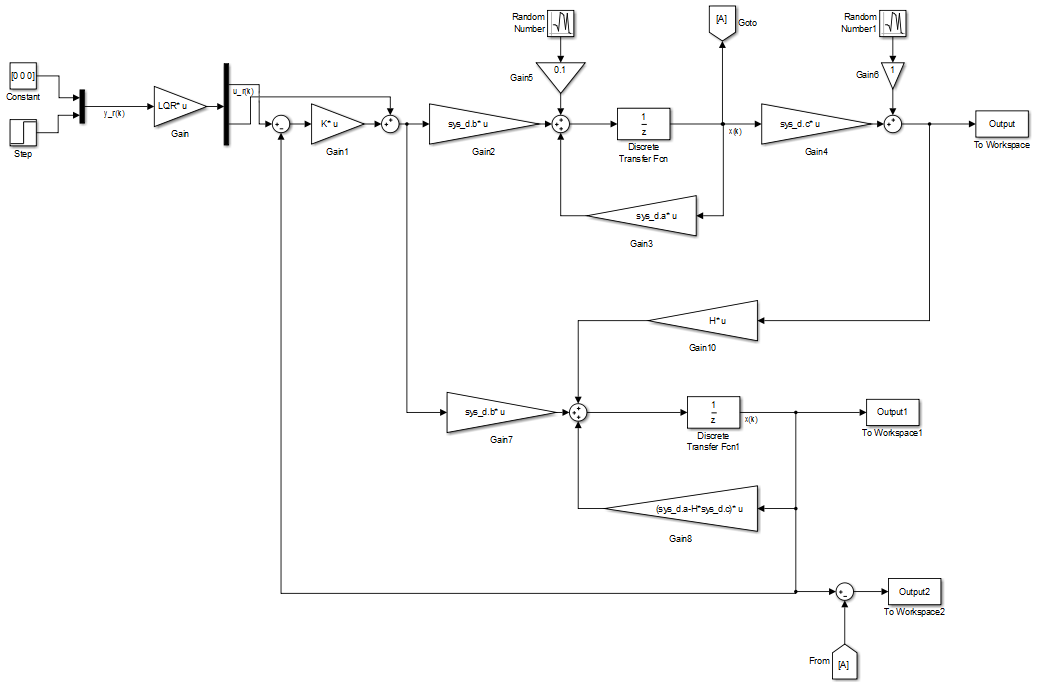
\includegraphics[width=0.9\linewidth]{images/model.png}
		\caption{Modelo del espacio de estados con observador.}
		\label{Model}
	\end{figure}
	\FloatBarrier
	%
	Para el calculo de la matriz $H$ para conseguir el filtro de Kalman se ha de hacer el siguiente proceso iterativo:
	
	\begin{myalign}
		\begin{split}
			H(k) &= (A \cdot P(k/k-1) \cdot C^t + R_{12})(C \cdot P(k/k-1) \cdot C^t + R_2)^{-1}\\
			x_e(k+1/k) &= A \cdot x_e(k/k-1) + B \cdot u(k) + H(k)(y(k)-C \cdot x_e(k/k-1))\\	
			P(k+1/k) &= A \cdot P(k/k-1) \cdot A^t + R_1 - H(k) \cdot (C \cdot P(k/k-1) \cdot A^t + R_{12}^t )
		\end{split}
	\end{myalign}
	%
	Partiendo de:
	\begin{myalign}
		\begin{split}
			&x_e(0)\\
			&P(0) = R_0
		\end{split}
	\end{myalign}
	
	En matlab este algoritmo se ejecuta de la siguiente forma:
	
	\begin{lstlisting}
	Const = 0.01;
	R_1 = Const * eye(3);
	R_12 = zeros(3,1);
	R_2 = Const * eye(1);
	Const1 = 1000;
	P = Const1 * eye(3);
	H = 0;
	H_save = 0;
	k = 0;
	
	while 1
		k = k + 1;
		H = (sys_d.a * P * sys_d.c' + R_12) * inv(sys_d.c * P * sys_d.c' + R_2);
		P = sys_d.a * P * sys_d.a' + R_1 - H * (sys_d.c * P * sys_d.a' + R_12');
		if ((H-H_save) < [0.001; 0.001; 0.001]) & (k > 30 )
			break;
		end
		H_save = H;
	end
	\end{lstlisting} 
	%
	Y se obtiene la siguiente matriz $H$:
	\begin{lstlisting}
	H =
	
	-0.7500
	0.0552
	0.6348
	\end{lstlisting}
	
	Esta matriz se lleva al modelo y se obtiene la salida del sistema de la Figura \ref{Output}.
	
	\begin{figure}[h!]
		\centering
		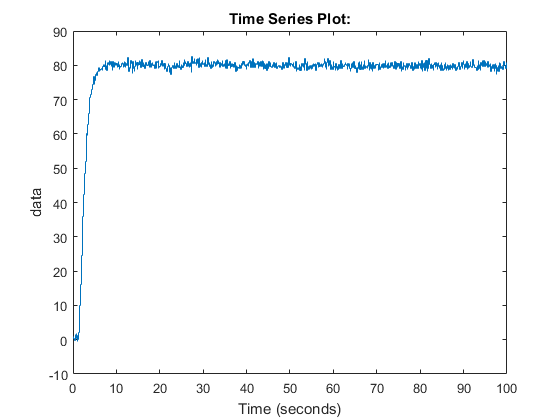
\includegraphics[width=0.8\linewidth]{images/output.png}
		\caption{Salida del sistema a controlar.}
		\label{Output}
	\end{figure}
	\FloatBarrier
	
	Si nos fijamos en la diferencia de los estados del sistema y del observador, se obtiene la Figura \ref{States}.
	
	La varianza de la diferencia de los estados es la siguiente:
	
	\begin{myalign}
		\begin{split}
			var(\dot{x}_{o1} - \dot{x}_1) &= 0.7019\\
			var(\dot{x}_{o2} - \dot{x}_2) &= 0.0553\\
			var(\dot{x}_{o3} - \dot{x}_3) &= 0.2001
		\end{split}
	\end{myalign}
	
	\begin{figure}[h!]
		\centering
		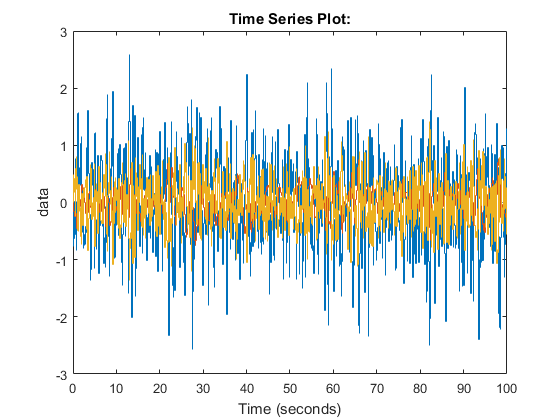
\includegraphics[width=0.8\linewidth]{images/states.png}
		\caption{Diferencia de los estados del sistema y del observador.}
		\label{States}
	\end{figure}
	\FloatBarrier
	
	Se calculan de la siguiente manera:
	
	\begin{lstlisting}
	var(Output2.Data(:,1));
	var(Output2.Data(:,2));
	var(Output2.Data(:,3));
	\end{lstlisting}
	
	
	
\end{document}